\chapter{Architecture Constraints}
\label{sec:constraints}
\section{Environment}
\label{sec:environment}
\input{generated/tables/tools.tex}

\section{Layers Definition}

\RequirementTag{SDD_SUSD}{143}
\\
\begin{figure}[H]
	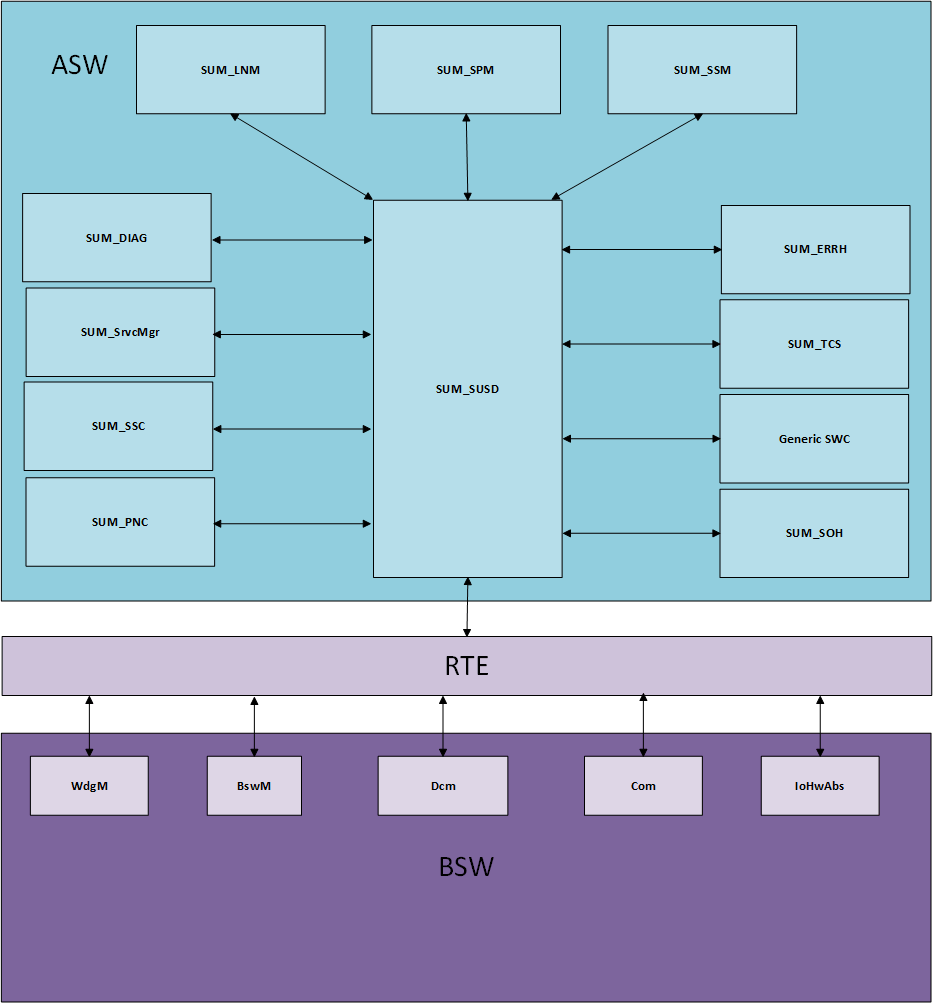
\includegraphics[width=\textwidth]{images/layers.png}
	\caption{SUSD layers}
	\label{fig:layers}
\end{figure}

The applied system architecture is based on Autosar v4.0.3. For detailed information on it refer to Autosar.org website.
\\
\Satisfies{SRS_SUSD 005}

\section{Generic component interface}

\begin{center}
	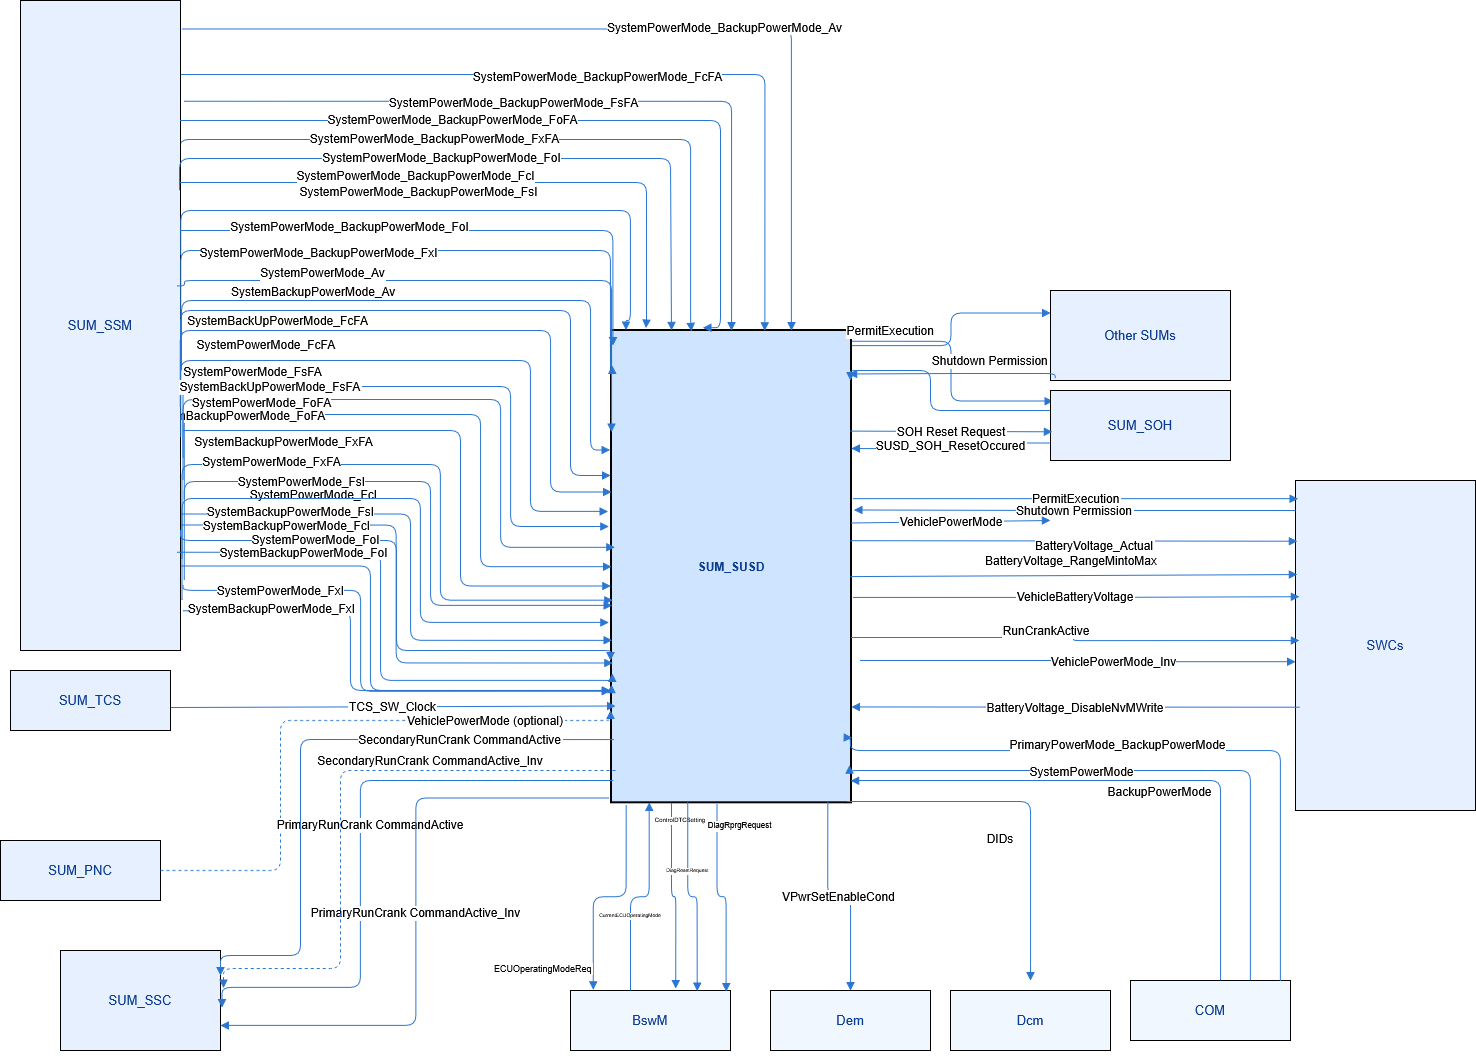
\includegraphics[width=\textwidth]{images/component}
	\label{sec:component}
\end{center}

\subsection{Port Interfaces}
\label{sec:port-interfaces}

\Requirement{001}
{}
{\Satisfies{SRS_SUSD 111} \Satisfies{SRS_SUSD 112} \Satisfies{SRS_SUSD 113} \Satisfies{SRS_SUSD 026} \Satisfies{SRS_SUSD 025} \Satisfies{SRS_SUSD 029} \Satisfies{SRS_SUSD 038} \Satisfies{SRS_SUSD 061} \Satisfies{SRS_SUSD 063} \Satisfies{SRS_SUSD 066} \Satisfies{SRS_SUSD 068} \Satisfies{SRS_SUSD 073} \Satisfies{SRS_SUSD 078} \Satisfies{SRS_SUSD 079} \Satisfies{SRS_SUSD 080} \Satisfies{SRS_SUSD 081} \Satisfies{SRS_SUSD 082} \Satisfies{SRS_SUSD 083} \Satisfies{SRS_SUSD 084} \Satisfies{SRS_SUSD 085} \Satisfies{SRS_SUSD 086} \Satisfies{SRS_SUSD 087} \Satisfies{SRS_SUSD 088} \Satisfies{SRS_SUSD 089} \Satisfies{SRS_SUSD 090} \Satisfies{SRS_SUSD 091} \Satisfies{SRS_SUSD 092} \Satisfies{SRS_SUSD 093} \Satisfies{SRS_SUSD 094} \Satisfies{SRS_SUSD 095} \Satisfies{SRS_SUSD 096} \Satisfies{SRS_SUSD 097} \Satisfies{SRS_SUSD 064} \Satisfies{SRS_SUSD 065} \Satisfies{SRS_SUSD 069} \Satisfies{SRS_SUSD 070} \Satisfies{SRS_SUSD 074} \Satisfies{SRS_SUSD 101} \Satisfies{SRS_SUSD 102} \Satisfies{SRS_SUSD 103} \Satisfies{SRS_SUSD 104} \Satisfies{SRS_SUSD 105} \Satisfies{SRS_SUSD 106} \Satisfies{SRS_SUSD 107} \Satisfies{SRS_SUSD 108} \Satisfies{SRS_SUSD 109} \Satisfies{SRS_SUSD 110} \Satisfies{SRS_SUSD 016} \Satisfies{SRS_SUSD 072} \Satisfies{SRS_SUSD 123} \Satisfies{SRS_SUSD 124} \Satisfies{SRS_SUSD 125} \Satisfies{SRS_SUSD 126} \Satisfies{SRS_SUSD 122} \Satisfies{SRS_SUSD 148} \Satisfies{SRS_SUSD 149} \Satisfies{SRS_SUSD 191} \Satisfies{SRS_SUSD 150} \Satisfies{SRS_SUSD 151} \Satisfies{SRS_SUSD 196} \Satisfies{SRS_SUSD 197} \Satisfies{SRS_SUSD 198} \Satisfies{SRS_SUSD 226} \Satisfies{SRS_SUSD 231} \Satisfies{SRS_SUSD 232} \Satisfies{SRS_SUSD 233} \Satisfies{SRS_SUSD 014} \Satisfies{SRS_SUSD 294} \Satisfies{SRS_SUSD 330}}
\input{generated/tables/port_interfaces.tex}

\Requirement{248}
{
For (FFI) compliance, all Sender-Receiver port interfaces connecting SUM\_SUSD to other RTA-SUM modules and SWCs shall be described in the Software Component Description (SWCD). This covers S/R P-ports provided to SUM\_SOH, SUM\_DIAG, SUM\_SSC, SUM\_SSM, SUM\_PNC, SUM\_SSFM, SUM\_TCS, SUM\_LNM, SUM\_ERRH, and SUM\_SPM (PermitExecution, VehiclePowerMode, BatteryVoltage\_Actual, DisableNVMWrite, RunCrankActive, RunCrankInput, SOH\_ResetOccurred interfaces), and S/R R-ports received from those modules (ShutdownPermission).
SUM\_SUSD SHALL be the \textit{only} owner of the writing operation for the specific interfaces in the SWCD.
}
{\Satisfies{SRS_SUSD 334} \Satisfies{rta_sum_ffi 001}}

\Requirement{249}
{
For (FFI) compliance, the Client-Server port interface between SUM\_SUSD (client) and SUM\_SPM (server) shall be described in the Software Component Description (SWCD). This covers the C/S R-port used by SUM\_SUSD to invoke the \texttt{ActivityRecordCmd} operation on SUM\_SPM.
SUM\_SUSD is the \textit{sole} caller of this operation: no other component in the system shall independently invoke \texttt{ActivityRecordCmd} on the same software composition, ensuring no interference between callers. SUM\_SUSD SHALL also verify the input values before invoking the C/S operation.
}
{\Satisfies{SRS_SUSD 334} \Satisfies{rta_sum_ffi 001} \Satisfies{rta_sum_ffi 002}}

\subsection{SUSD DID services to Dcm}
\label{sec:DID}

\Requirement{002}
{}
{\Satisfies{SRS_SUSD 076} \Satisfies{SRS_SUSD 077} \Satisfies{SRS_SUSD 114} \Satisfies{SRS_SUSD 117} \Satisfies{SRS_SUSD 118} \Satisfies{SRS_SUSD 119} \Satisfies{SRS_SUSD 120} \Satisfies{SRS_SUSD 121} \Satisfies{SRS_SUSD 262} \Satisfies{SRS_SUSD 275} \Satisfies{SRS_SUSD 277} \Satisfies{SRS_SUSD 330}}
\input{generated/tables/DID.tex}

\subsection{SUSD RID services}
\label{sec:RID}
\Requirement{150}
{\input{generated/tables/RID.tex}}
{\Satisfies{SRS_SUSD 263} \Satisfies{SRS_SUSD 278} \Satisfies{SRS_SUSD 279}}

\section{Other constraints and assumptions}

\subsection{Assumptions}
\label{sec:assumptions}
\Requirement{159}
{}
{\Satisfies{SRS_SUSD 264} \Satisfies{SRS_SUSD 265} \Satisfies{SRS_SUSD 266} \Satisfies{SRS_SUSD 267} \Satisfies{SRS_SUSD 268} \Satisfies{SRS_SUSD 269}}
\begin{enumerate}
\item The modes indicated to BswM through \code{ECUOperatingModeReq} interface will be values of the type \DatatypeRef{CurrentECUOperatingModeType}.
\item Timers \ConfigurationParameterRef{SUSD_t_Shutdown_Refresh} and \ConfigurationParameterRef{SUSD_t_Force_Shutdown_Wait} shall be used for both SUMs and SWCs.
\item SUSD shall go ahead with Shutdown Permission indication from only 8 SUMs (PNC, ERRH, SOH, LNM, TCS, SSC, SSM and SrvcMgr) on Reset.
\item SUM_SUSD shall store ECU Wakeup reason (list of wakeups) information along with the time of occurrence of this event in to NvM.
The time of occurrence shall be calculated by using \code{TCS_SWC_Clock} from SUM_TCS.
\item \code{SUSD_HardwareReady} function is provided for user to provide the information regarding the availability of hardware.
\item \code{ControlDTCSetting} is used to determine whether to report errors (resulting from comparing the termination) to Dem or not and it shall be mode switch interface.
\item The CompuMethod has been created for Run Crank Input Type \code{SUSD_DISCRETE} and \code{SUSD_ANALOG} to consider Run Crank Input Type as Enum and \code{SUSD_DISCRETE} is considered as default.
\item \code{VehicleBatteryVoltage} input to SUSD and \code{BatteryVoltage_Actual} output from SUSD are  \code{uint8} datatype with Range as 3V to 25V only.
\item An ECU shall store its wakeup reasons per the AUTOSAR State Manager Specification and SDV-8002.
\item In addition to the requirements in the AUTOSAR ECU State Manager Specification, an ECU can store any additional supplier specific reasons. All of the possible wakeup reasons are not required to be supported. If any of these wakeup reasons are supported they shall be defined in the bit location shown in DID F09E.
\item AUTOSAR allows up to 32 total wakeup reasons to be defined and stored. The first 16 (bits 0-15) are globally defined wakeup sources; the remaining 16 (bits 16-31) are ECU-specific/supplier defined wakeup sources.
\item See DID 0xF09E: ECU Wakeup Detection Records for source name detail.
\item Supplier defined wakeups (controller specific) shall be approved by GM and documented in the ECU CTRS and ECU Diagnostic Specification.
\item An ECU shall provide sufficient non-volatile memory to store the 10 most recent wakeup records (Records 1 to 10 recorded as a push down stack (PDS)).
\end{enumerate}

\subsection{Constraints}
\label{sec:constraints}

\begin{enumerate}
\item Runnable \RunnableRef{RE_SUSD_RunCrankManagement} shall be executed before \RunnableRef{RE_SUSD_VehiclePowerMode}.
\item On wakeup, all SWCs shall be indicated through Permit Execution interface, mapping of SWCs to wakeup is not considered.
\item \code{NvM_WriteAll()} will be done for \code{SUSD_WakeUpSrcTimeInfo} by NvM module.
\end{enumerate}